% Nallino, Part I p. 64: the circles of a planet, redrawn from the print: the circle ABCD (parecliptic),
% the circle GBFD (deflecting, centre E), the excentric GHKL (centre M), the epicycles PQS (centre H)
% and RVX (centre L), the diameter AF and the lines MHQ, EHP, ETN, MLR, ELV and EXZ. Circles and
% lines are least-squares fits to the printed ink; coordinates are PDF points of master page 153
% less the origin (111.6, 267.67), y downward.
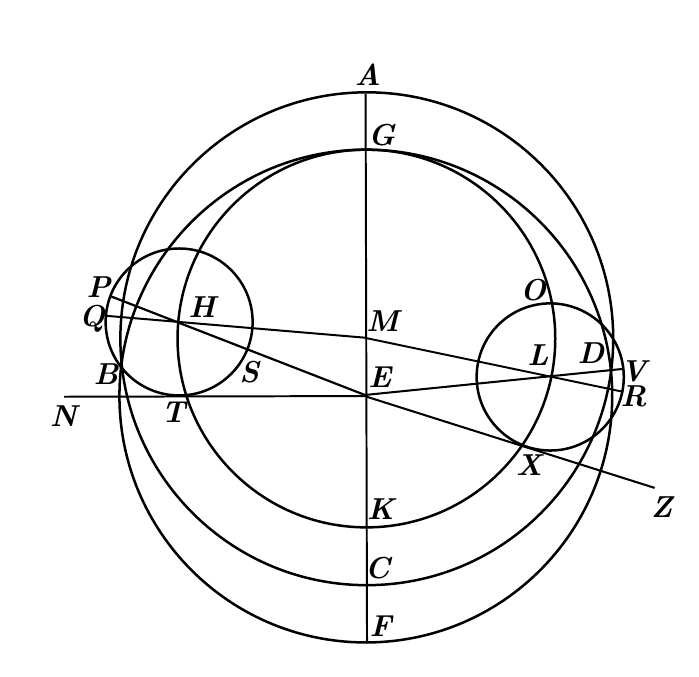
\begin{tikzpicture}[x=0.9886pt,y=-0.9886pt,line cap=butt,every node/.style={font=\fontsize{10.5}{10.5}\bfseries\itshape\selectfont,inner sep=0pt}]
\useasboundingbox (0,0) rectangle (235.00,227.00);
\draw[line width=0.90pt] (123.95,113.70) circle[radius=90.07];  % the circle ABCD (parecliptic)
\draw[line width=0.91pt] (123.60,134.65) circle[radius=90.06];  % the circle GBFD (deflecting), centre E
\draw[line width=0.90pt] (123.81,113.62) circle[radius=69.03];  % the excentric GHKL, centre M
\draw[line width=0.90pt] (55.36,107.57) circle[radius=26.86];  % the epicycle PQS, centre H
\draw[line width=0.91pt] (191.00,127.67) circle[radius=26.89];  % the epicycle RVX, centre L
\draw[line width=0.71pt] (123.51,24.20) -- (124.04,225.08);  % the diameter AF through the centres
\draw[line width=0.72pt] (123.74,113.35) -- (28.59,105.31);  % M through H to Q
\draw[line width=0.80pt] (123.80,134.46) -- (30.21,98.13);  % E through H to P
\draw[line width=0.71pt] (13.29,134.90) -- (123.80,134.65);  % E through T to N
\draw[line width=0.70pt] (123.74,113.46) -- (217.67,133.10);  % M through L to R
\draw[line width=0.74pt] (123.80,134.21) -- (217.96,124.69);  % E through L to V
\draw[line width=0.74pt] (123.80,134.86) -- (229.17,168.22);  % E through X to Z
\node at (124.30,17.33) {A};
\node at (129.40,39.23) {G};
\node at (25.90,94.85) {P};
\node at (23.50,106.63) {Q};
\node at (63.70,102.24) {H};
\node at (129.70,107.22) {M};
\node at (184.70,95.93) {O};
\node at (186.48,119.80) {L};
\node at (205.82,119.07) {D};
\node at (221.39,125.69) {V};
\node at (221.48,134.64) {R};
\node at (28.65,126.46) {B};
\node at (80.97,126.01) {S};
\node at (128.71,127.55) {E};
\node at (13.07,141.86) {N};
\node at (53.25,140.47) {T};
\node at (183.27,159.79) {X};
\node at (231.70,175.13) {Z};
\node at (129.07,175.92) {K};
\node at (127.81,197.55) {C};
\node at (128.98,218.79) {F};
\end{tikzpicture}
